% !TEX TS-program = pdflatex
% !TEX encoding = UTF-8 Unicode

% This is a simple template for a LaTeX document using the "article" class.
% See "book", "report", "letter" for other types of document.

\documentclass[12pt]{article} % use larger type; default would be 10pt
\usepackage[utf8]{inputenc}   % set input encoding (not needed with XeLaTeX)

%%% PAGE DIMENSIONS
\usepackage{geometry}
\geometry{a4paper}
\geometry{margin=1in} % 1in page margin

%%% COLOR AND GRAPHICS
\usepackage{color}
\usepackage{graphicx} % support the \includegraphics command and options

\usepackage{pslatex}
\definecolor{mygreen}{rgb}{0,0.6,0}
\definecolor{mygray}{rgb}{0.5,0.5,0.5}
\definecolor{mymauve}{rgb}{0.58,0,0.82}
\usepackage{listings} % For displaying source code
\lstset{ %
  language=C,                      % the language of the code
  backgroundcolor=\color{white},   % choose the background color; you must add \usepackage{color} or \usepackage{xcolor}
  basicstyle=\sffamily\fontsize{11}{13.2}\selectfont,        % the size of the fonts that are used for the code
  breakatwhitespace=false,         % sets if automatic breaks should only happen at whitespace
  breaklines=true,                 % sets automatic line breaking
  captionpos=t,                    % sets the caption-position to bottom
  commentstyle=\color{mygreen},    % comment style
  deletekeywords={...},            % if you want to delete keywords from the given language
  escapeinside={\%*}{*)},          % if you want to add LaTeX within your code
  extendedchars=true,              % lets you use non-ASCII characters; for 8-bits encodings only, does not work with UTF-8
  frame=single,                    % adds a frame around the code
  keepspaces=true,                 % keeps spaces in text, useful for keeping indentation of code (possibly needs columns=flexible)
  keywordstyle=\color{blue},       % keyword style
  morekeywords={*,...},            % if you want to add more keywords to the set
  numbers=left,                    % where to put the line-numbers; possible values are (none, left, right)
  numbersep=5pt,                   % how far the line-numbers are from the code
  numberstyle=\color{mygray},      % the style that is used for the line-numbers
  rulecolor=\color{black},         % if not set, the frame-color may be changed on line-breaks within not-black text (e.g. comments (green here))
  showspaces=false,                % show spaces everywhere adding particular underscores; it overrides 'showstringspaces'
  showstringspaces=false,          % underline spaces within strings only
  showtabs=false,                  % show tabs within strings adding particular underscores
  stepnumber=1,                    % the step between two line-numbers. If it's 1, each line will be numbered
  stringstyle=\color{mymauve},     % string literal style
  tabsize=2,                       % sets default tabsize to 2 spaces
  title=\lstname                   % show the filename of files included with \lstinputlisting; also try caption instead of title
}

% \usepackage[parfill]{parskip} % Activate to begin paragraphs with an empty line rather than an indent

%%% PACKAGES
\usepackage{booktabs} % for much better looking tables
\usepackage{array}    % for better arrays (eg matrices) in maths
\usepackage{paralist} % very flexible & customisable lists (eg. enumerate/itemize, etc.)
\usepackage{verbatim} % adds environment for commenting out blocks of text & for better verbatim
\usepackage{subfig}   % make it possible to include more than one captioned figure/table in a single float

%%% HEADERS & FOOTERS
%\usepackage{fancyhdr} % This should be set AFTER setting up the page geometry
%\pagestyle{fancy} % options: empty , plain , fancy
%\renewcommand{\headrulewidth}{0pt} % customise the layout...
%\lhead{}\chead{}\rhead{}
%\lfoot{}\cfoot{\thepage}\rfoot{}


%%% SECTION TITLE APPEARANCE
\usepackage{sectsty}
\sectionfont{\normalsize\bfseries\uppercase}
\subsectionfont{\normalsize\bfseries}
\subsubsectionfont{\normalsize\mdseries\itshape}

%%% ToC (table of contents) APPEARANCE
\usepackage[nottoc,notlof,notlot]{tocbibind} % Put the bibliography in the ToC
\usepackage[titles,subfigure]{tocloft} % Alter the style of the Table of Contents
\renewcommand{\cftsecfont}{\rmfamily\mdseries\upshape}
\renewcommand{\cftsecpagefont}{\rmfamily\mdseries\upshape} % No bold!

%%% Title setup
\newcommand{\TitleFont}{\fontsize{16}{20}\selectfont\bfseries}
\newcommand{\AuthorFont}{\fontsize{14}{17}\selectfont}

%%% END Article customizations

%%% The "real" document content comes below...

\title{\TitleFont EE 472 Lab 1 \\ Introducing the Lab Environment \vfill }
\author{\AuthorFont Jonathan Ellington \\ Patrick Ma \\ Jarrett Gaddy}
\date{}

\begin{document}

%% Make title and ToC, start page numbering AFTER ToC
\maketitle
\thispagestyle{empty}
\pagebreak
\tableofcontents
\listoftables
\listoffigures
\thispagestyle{empty}
\pagebreak
\setcounter{page}{1}

\section{Abstract}
The abstract should provide a brief overview of the report.  It should provide a summary of the main specific points for the introduction, the main tests and experiments, the results, and the conclusions. It is called an abstract because you can literally "abstract" sentences from the other sections. 

Once again, this is not a narrative of your experiences as you executed the design.  The abstract should mirror (albeit in a very condensed way) the content of your report.

\section{Introduction}
\textbf{Brief introduction and overview of the purpose of the lab and of the methods and tools used.}

\section{Discussion of the Lab}

This section should include the following:

\subsection{Design Specification  Patrick}

\textbf{In this subsection you will textually describe your client's requirements.  What does he or she need in the project you are developing.  If you are incorporating extra features or capabilities, please describe them clearly in this section.i}

The entire system must satisfy several lofty objectives. The final product must be portable, lightweight, and internet enabled. The system must also make measurements of vital bodily functions, perform simple computations, provide datalogging functionality, and indicate when measured vitals exceed given ranges, or the user fails to comply with a prescribed logging regimen. \\
At the present time, only two subsystems must be produced: the display and alarm portions. Additionally, the system must demonstrate the ability to store basic measurements. The initial functional requirements for the system are: 

\begin{itemize}[$$]
  \item The initial functional requirements for the system are:

    \begin{itemize}[$\bullet$]
      \item Provide continuous sensor monitoring capability
      \item Produce a visual display of the sensor values
      \item Accept variety of input data types
      \item Provide visual indication of warning states
      \item Provide an audible indicator of alarm states
    \end{itemize}
\end{itemize}

\begin{itemize}[$$] 
  \item The system must have the following outputs:
    \begin{itemize}[$\bullet$]
      \item Display of measured vitals and battery status
      \item Visual signals for three battery states
      \item Visual signal of low battery state
      \item Audio signal of alarm state
    \end{itemize}
\end{itemize}

\begin{itemize}[$$]
  \item The system must have the following inputs:
    \begin{itemize}[$\bullet$]
      \item Alarm acknowledgement capability
      \item Sensor measurement input capability
    \end{itemize}
\end{itemize}


\begin{itemize}[$$]
  \item Overall summary description of the module - 2-3 paragraphs maximum (explanation of use cases goes here)

    \begin{itemize}[$$]
      \item Specification of the public interface to the module

        \begin{itemize}[$\bullet$]
          \item Inputs
          \item Outputs
          \item Side effects
        \end{itemize}

      \item Psuedo English description of algorithms, functions, or procedures
      \item Timing constraints
      \item Error handling
    \end{itemize}
\end{itemize}

\begin{table}[h]
    \centering
    \label{table:ex}
    \begin{tabular}{llr}
        \toprule
        Animal    & Description & Price (\$) \\
        \midrule
        Gnat      & per gram    & 13.65      \\
                  & each        & 0.01       \\
        Gnu       & stuffed     & 92.50      \\
        Emu       & stuffed     & 33.33      \\
        Armadillo & frozen      & 8.99       \\
        \bottomrule
    \end{tabular}
    \caption{Example table.}
\end{table}

\subsection{Software Implementation  Jon}


\subsubsection{Top level design Jon}

%- User use cases  (need to fix)
%  + Take measurements
%  + Acknowledge alarm
%- High level blocks
%  + Functional decomposition
%    o User
%    o Stellaris board
%    o External Sensors
%  + System Architecture (need to flip inheritance arrows and composition arrow)
%    o Discuss shared data
%    o Discuss TCB->Schedular composition
%    o Discuss TCB->task inheritance
%    o Interaction with hardware
%- Implementation in C
%  + Scheduler
%    o Has queue of TCBs
%    o Runs each with minor cycle delay
%      - Timebase
%        o Specifies major/minor cycle
%  + Tasks
%    o Global data is declared in a header file, globals.h and shared with everyone
%    o Get their own file and header file
%    o Own data is hidden from rest of program, single pointer exposed
%    o Every task gets an initialization to initialize data

The design process began by identifying the use cases and actors involved with the system.  In the specified system, the user interacts with the system in one of two ways:
\begin{enumerate}
  \item The user can view their vitals
  \item The user will acknowledge an alarm condition to silence the alarm
\end{enumerate}
In order for a user to view their vitals, the system will have to interact with some external sensors.  Specifically, the system will interact with blood pressure, temperature, and pulse rate sensors.  A graphical depiction of this is shown in Figure~\ref{fig:use}.

\begin{figure}
    \centering
    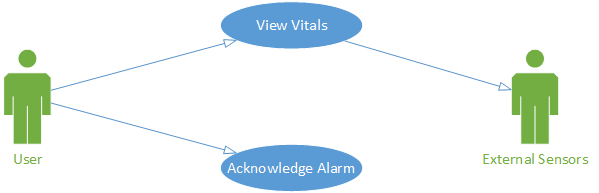
\includegraphics[width=\textwidth]{../design/use_cases_graphical}
    \caption{Use-Case Diagram}
    \label{fig:use}
\end{figure}

After understanding how the user would interact with the device, the system was
functionally decomposed into high-level blocks as shown in
Figure~\ref{fig:func}.  The main system control is located in the CPU, which
controls all data flow into and out of the peripheral devices.  The OLED
displays the user's current vitals including blood pressure (systolic and
diastolic), temperature, and pulse rate.  In the future external sensors will
be added, but for now the values are simulated using the CPU.  The CPU also
controls three LEDs colored green, yellow, and red.  These LEDs are used to
inform the user on the current state of their vitals as well as the state of
the device.  Under normal circumstances, the green LED will be lit.  If the
users' vitals fall outside of a specified range, the red LED will flash at a
specified rate, dependant on which vital is out of range.  If the battery is
low, the yellow LED will be illuminated.

\begin{figure}[h]
    \centering
    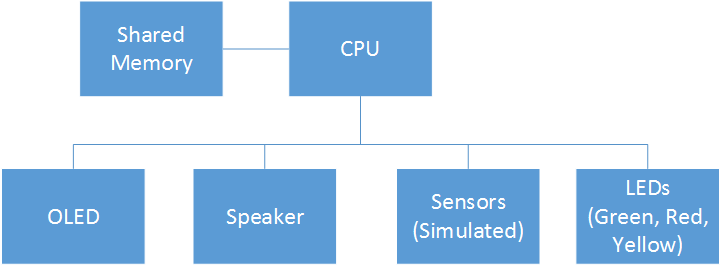
\includegraphics[width=\textwidth]{../design/Functional_decomposition}
    \caption{Functional Decomposition}
    \label{fig:func}
\end{figure}

Next, the system architecture was developed (Figure~\ref{fig:arch}).  At a high
level the system works on two main concepts, the scheduler and tasks.  Tasks
embody some sort of work being done, and the scheduler is in charge of
determining the speed and order in which the tasks execute.  The system has
several tasks, each with their own specific job.  For modularity reasons, each
task should have the same public interface and the scheduler should be able to
run each task regardless of that specific tasks job or implementation.  Thus
the task concept is abstracted into a Task Control Block (TCB), and the
scheduler maintains a queue of TCBs to run.  The TCB abstraction is shown in
Figure~\ref{fig:arch} using inheritance, and the fact that the scheduler has a
queue of TCBs is shown with composition.  The core functionality of the system
was divided into the following five main tasks:
\begin{itemize}
  \item \textbf{Measure Task} - In charge of interacting with the blood pressure, temperature, and pulse sensors (simulated)
  \item \textbf{Compute Task} - Converts sensor data into human readable format
  \item \textbf{Display Task} - Displays the measurements on the Stellaris OLED
  \item \textbf{Warning/Alarm Task} - Interacts with the red, yellow, and green LEDs, as well as the speaker to annunciate warning and alarm information
  \item \textbf{Status Task} - Receives battery information from the device
\end{itemize}
Each of these tasks interact using the shared data shown in Figure~\ref{fig:arch}. 

\begin{figure}
    \centering
    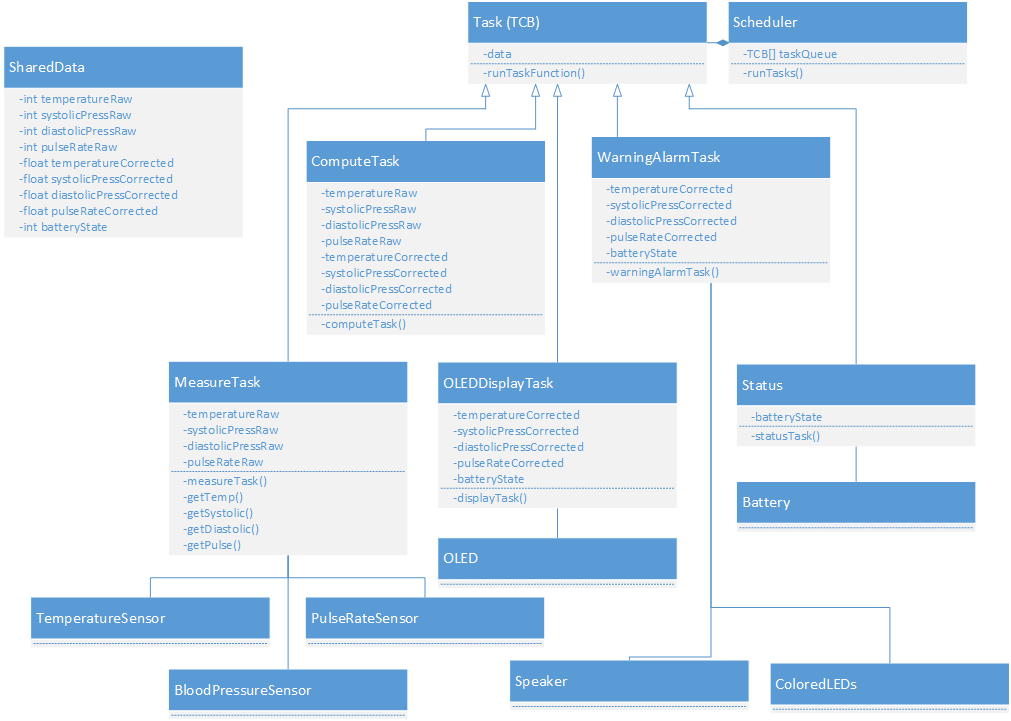
\includegraphics[width=\textwidth]{../design/System_Architecture}
    \caption{System Architecture Diagram}
    \label{fig:arch}
\end{figure}

After developing the system architecture, the design needed to be translated into the C programming language.  The design manifested in a multifile program consisting of the following source files:
\begin{itemize}
  \item \textbf{globals.c/globals.h} - Used to define the Shared Data used among the tasks
  \item \textbf{schedule.c/schedule.h} - Defines the scheduler interface and it's implementation, as well as the TCB structure
  \item \textbf{timebase.h} - Defines the timebase used for the scheduler and tasks
\end{itemize}
Each task also has it's corresponding ``.c'' and ``.h'' file (for example, measure.c and measure.h).

The TCB structure that the scheduler uses must work for all tasks, and must not
contain any task-specific information.  Instead, the TCB consists of only a void pointer to the tasks data, and a pointer to a function that returns void and takes a void pointer, as follows:
\begin{lstlisting}
struct TCB {
  void *taskDataPtr;
  void (*taskRunFn)(void *);
}
\end{lstlisting}
Leaving out the type information allows the scheduler to pass the task's data
(*taskDataPtr) into the task's run function completely unaware of the kind of
data the task uses or how the task works.

For increased modularity, the data structure used by each task was not put in
the task's header file.  Instead, the structure was declared within the task
implementation file, and instantiated using a task initialization function.  In
the header file, a void pointer pointing to the initialized structure is
exposed with global scope, as well as the task's run and initialization functions.

\subsubsection{low level design  Jarret}

implementation details here. Tasks, scheduler, etc. Control diagram goes here, activity diagram, etc.

\section{Presentation, Discussion, and Analysis of the Results}

Based upon the execution of your design, present your results. Explain them and what was expected, and draw any conclusions (for example, did this prove your design worked).

In addition to a detailed discussion and analysis of your project and your results, you must include all the answers to all questions raised in the lab.
\subsection{results  patrick}

\subsection{discussion of results  Jon}

\subsection{Analysis of any Errors  Patric}

This one is obvious. Do this section as appropriate.  If it improves the flow, it does not need to be a separate section and may be included in the presentation, discussion, and analysis of the results.  However, it will still be graded separately and must be present.

\subsection{Analysis of problems and issues encountered and what efforts were made to identify the root cause of any problems  Jarrett}

State any problems you encountered while working on the project. If your project did not work or worked only partially, provide an analysis of why and what efforts were made to identify the root cause of any problems. \\

Some points to bring up: did not enable the GPIO bank (caused OLED display to not work), could not get switch to work (solved by understanding that switch required pull up). P or J can talk about design solutions that did not work. On the whole, we had problems with going too deep, too quickly.

\section{Test Plan Patrick}

Overall summary of what needs to be tested to ensure that your design meets the original requirements, 2-3 paragraphs maximum unless specified otherwise

\subsection{Test Specification}

Annotated description of what is to be tested and the test limits.  This specification quantifies inputs, outputs, and constraints on the system.  That is, it provides specific values for each. 

Note, this does not specify test implementation...this is what to do, not how to do it.

\subsection{Test Cases  Jarrett}

Annotated description of how your system is to be tested against the test limits
Note, this does specify test implementation...this is not what to do, this is how to do it based upon the test specification.

\section{Summary and Conclusion}

You should know these sections very well, no need to explain.  Note, however, that they are two different sections.  The summary is just that, a summary of your project.  It should loosely mirror the abstract with a bit more detail.  The conclusion concludes the report, potentially adds information that is often outside the main thrust of the report, and may offer suggestions or recommendations about the project.

\subsection{Final Summary}


\subsection{Project Conclusions}


\pagebreak
\appendix

\section{Source Code}

Source code for this project is provided below.

\subsection{The first part}
% \lstinputlisting{source.c}

\subsection{The second part}
% \lstinputlisting{source.c}

\end{document}
